%!TEX root = main.tex

\chapter{Basic graphing in Python}\label{appendix:matplotlib}

One of the advantages of doing scientific computing with Python is the wealth of different libraries we may use to represent data and functions graphically.  In this appendix we are going to do a quick overview of some of the most widely used:

\begin{enumerate}
	\item \matplotlib
	\item \texttt{bokeh}
	\item \texttt{plotly}
\end{enumerate}

\section{\matplotlib}

The \matplotlib\ libraries are fundamentally focused on 2D plotting.  They are open source with license based on the \emph{Python Software Foundation} (PSF) license.  If you are planning to use them for your scientific production, it is customary to cite John Hunter's 2007 seminal paper \cite{Hunter:2007}.   

In this section we are going to explore just a handful of utilities:
\begin{itemize}
 	\item The module \pyplot, that allows us to use a similar syntax and interface as in \texttt{matlab} or \texttt{octave}
 	\item The toolkit \texttt{mplot3d} to extend \matplotlib\ for simple 3D plotting.
 	\item The toolkits \texttt{basemap} and \texttt{cartopy} to extend \matplotlib\ for projection and Geographic mapping.
 	\item The toolkit \texttt{ggplot} for those of you familiar with the \texttt{R} plotting system.
 \end{itemize} 

Let's start with a simple example or usage of the module \pyplot.  We are going to use exclusively the Rosenbrock function $\mathcal{R}_{1,1}$.

\begin{minted}[frame=single, fontsize=\footnotesize, linenos, mathescape]{python}
import numpy as np, matplotlib.pyplot as plt 

def R(x,y): return (1.0-x)**2 + (y - x**2)**2
\end{minted}

For each plot, we usually indicate in our session the intent to create a \emph{figure}.  At that point it is customary to impose the size of the figure, number of subplots (if more than one), kind of axis, usage of grid, etc.  This is what we call the \emph{layout} of our diagrams.  For instance, to create a simple plot (with size $5 \times 10.5$) of the graph of $f(x) = \mathcal{R}(x,1)$ for $-2 \leq x \leq 2$, but focusing only in the window $[-2.5,2.5] \times [-0.5, 10]$, we issue the following commands:

\begin{minted}[frame=single,fontsize=\footnotesize, mathescape]{python}
>>> x = np.linspace(-2, 2)         # $-2 \leq x \leq 2$

>>> plt.figure(figsize=(5,10.5));  # Create a figure of requested size
... plt.axes(aspect='equal');      # I want x's and y's to be the same size
... plt.grid();                    # I want a grid
... plt.xlim(-2.5, 2.5);           # Set my window
... plt.ylim(-0.5, 10);
... plt.plot(x, R(x,1.0));         # Just plot it...
... plt.show()                     # ...and request it shows in screen
\end{minted}

See Figure \ref{figure:basicplt}, left.

It is possible to combine several plots on the same figure:

\begin{minted}[frame=single,fontsize=\footnotesize, mathescape]{python}
>>> plt.figure(figsize=(5,10.5));
... plt.axes(aspect='equal');  
... plt.grid();
... plt.xlim(-2.5, 2.5);
... plt.ylim(-0.5, 10);
... for section in range(1,6):     # Do 5 plots: R(x,n)
...     plt.plot(x,R(x,section))   # where n=1,2,3,4,5
...
... plt.show()
\end{minted}

See Figure \ref{figure:basicplt}, center.

It is hard to see which graph corresponds to which function, in spite of the different chosen colors.  We solve this issue this by allowing each graph to be labeled, and placing a legend in the diagram:

\begin{minted}[frame=single,fontsize=\footnotesize, mathescape]{python}
>>> plt.figure(figsize=(5,10.5));
... plt.axes(aspect='equal');  
... plt.grid();
... plt.xlim(-2.5, 2.5);
... plt.ylim(-0.5, 10);
... for section in range(1,6):     # The labels go here
...     plt.plot(x,R(x,section), label=section)  
...
... plt.legend()                   # The legend is requested here
... plt.show()
\end{minted}

See Figure \ref{figure:basicplt}, right.

\begin{figure}[ht!]
\begin{tabular}{ccc}
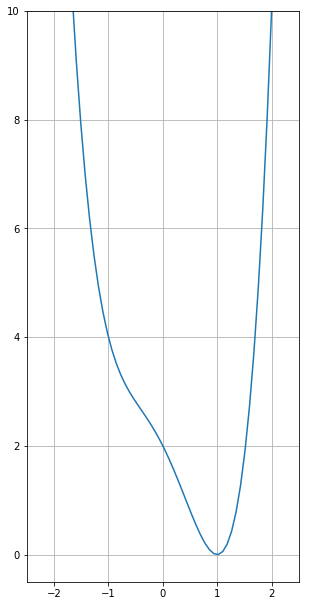
\includegraphics[width=0.33\linewidth]{images/basicplt.png} &
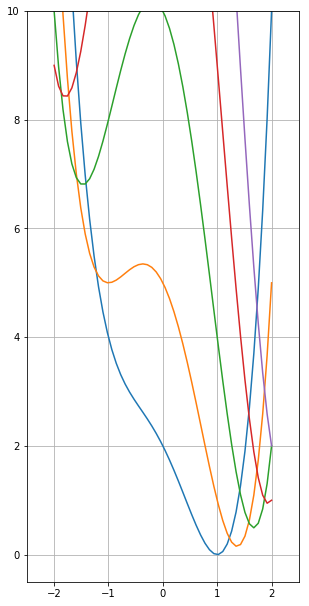
\includegraphics[width=0.33\linewidth]{images/4plotsplt.png} &
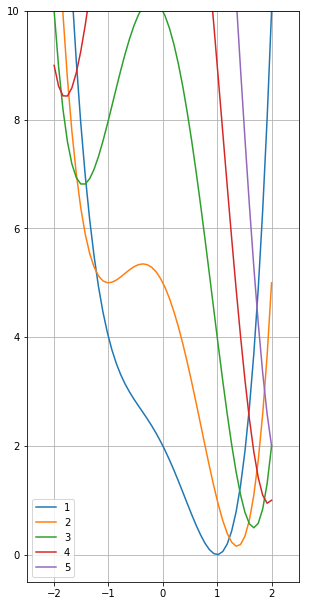
\includegraphics[width=0.33\linewidth]{images/4plotslegendplt.png}
\end{tabular}
\caption{Basic rendering of functions with \pyplot}
\label{figure:basicplt}
\end{figure}

It is possible to control more detail of your plots.  See for example how we modify line width, type, color, etc.  As an exercise, try to comment each line indicating what modifications have been performed on the corresponding graphs.

\begin{minted}[frame=single,fontsize=\footnotesize, mathescape]{python}
>>> plt.figure();                  # Let pyplot choose size and layout
... plt.plot(x, R(x,1), 'r-', lw=0.5);
... plt.plot(x, R(x,2), 'b--',lw=2);
... plt.plot(x, R(x,3), 'go');
... plt.plot(x, R(x,4), 'y-.');
... plt.show()
\end{minted}

\begin{figure}[ht!]
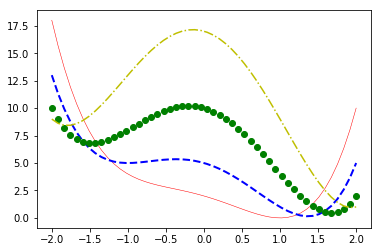
\includegraphics[width=0.75\linewidth]{images/intermediateplt.png}
\caption{Tinkering with color, style and width of lines in \pyplot}
\label{figure:intermediateplt}
\end{figure}

To plot a set of level lines (a countour plot), we can either do that manually, or request \pyplot\ to do it for us.  For instance to render the level lines $\mathcal{R}_{1,1}(x,y)=c$ for $c=1,2,3,5,10,15,20$ over the window $[-2,2] \times [-2,3]$, we could issue the following commands:

\begin{minted}[frame=single,fontsize=\footnotesize, mathescape]{python}
>>> y = np.linspace(-2,3)          # $-2 \leq y \leq 3$
>>> X,Y = np.meshgrid(x,y)         # generate the window

>>> plt.figure();                  # Let pyplot choose size and layout
... plt.contour(X, Y, R(X,Y), levels=[1,2,3,5,10,15,20]);
... plt.show()
\end{minted}

See Figure \ref{figure:contourplt}, left.

Although each level line has been rendered with a different color, it is hard to see which one is which.  Placing a legend on an already cluttered diagram may not be the best option.  Fortunately, there is a neat method to display relevant information of top of each level line:

\begin{minted}[frame=single,fontsize=\footnotesize, mathescape]{python}
>>> plt.figure();                  # Let pyplot choose size and layout
... CS = plt.contour(X, Y, R(X,Y), levels=[1,2,3,5,10,15,20]);
... plt.clabel(CS, fontsize=9, inline=1);
... plt.show()
\end{minted}

See Figure \ref{figure:contourplt}, right.

\begin{figure}[ht!]
\begin{tabular}{cc}
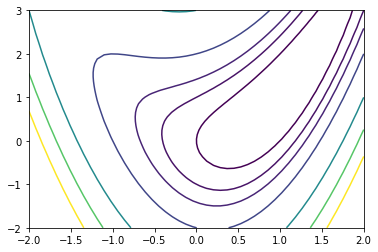
\includegraphics[width=0.5\linewidth]{images/contourplt.png} &
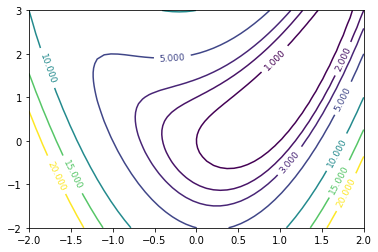
\includegraphics[width=0.5\linewidth]{images/contourplusplt.png}
\end{tabular}
\caption{Contour plots with \pyplot}
\label{figure:contourplt}
\end{figure}